\section{Realisering}
Kredsløbene fra analysen og simuleringen opbygges og måles i laboratoriet med oscilloskop. Figurerne nedenfor viser de fysiske måleopstillinger. 

\begin{figure}
\begin{center}
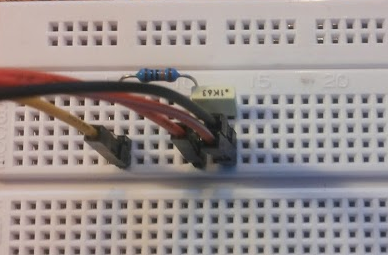
\includegraphics[height=5cm]{E_Fig/Rea_1_100}
\caption{Lavpasfilter R: 100 k$Omega$, C = 100nF
\label{Rea_1_100}
\end{center}
\end{figure}

\begin{figure}
\begin{center}
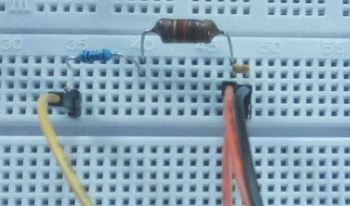
\includegraphics[height=5cm]{E_Fig/Rea_2_1}
\caption{Lavpasfilter R=1k$Omega$, =1mH, C=1nF}
\label{Rea_2_1}
\end{center}
\end{figure}

\subsection{Realisering af 1. ordens lavpasfilter}

\subsubsection{1k$Omega$}

\subsubsection{100k$Omega$}

\begin{figure}
\begin{center}
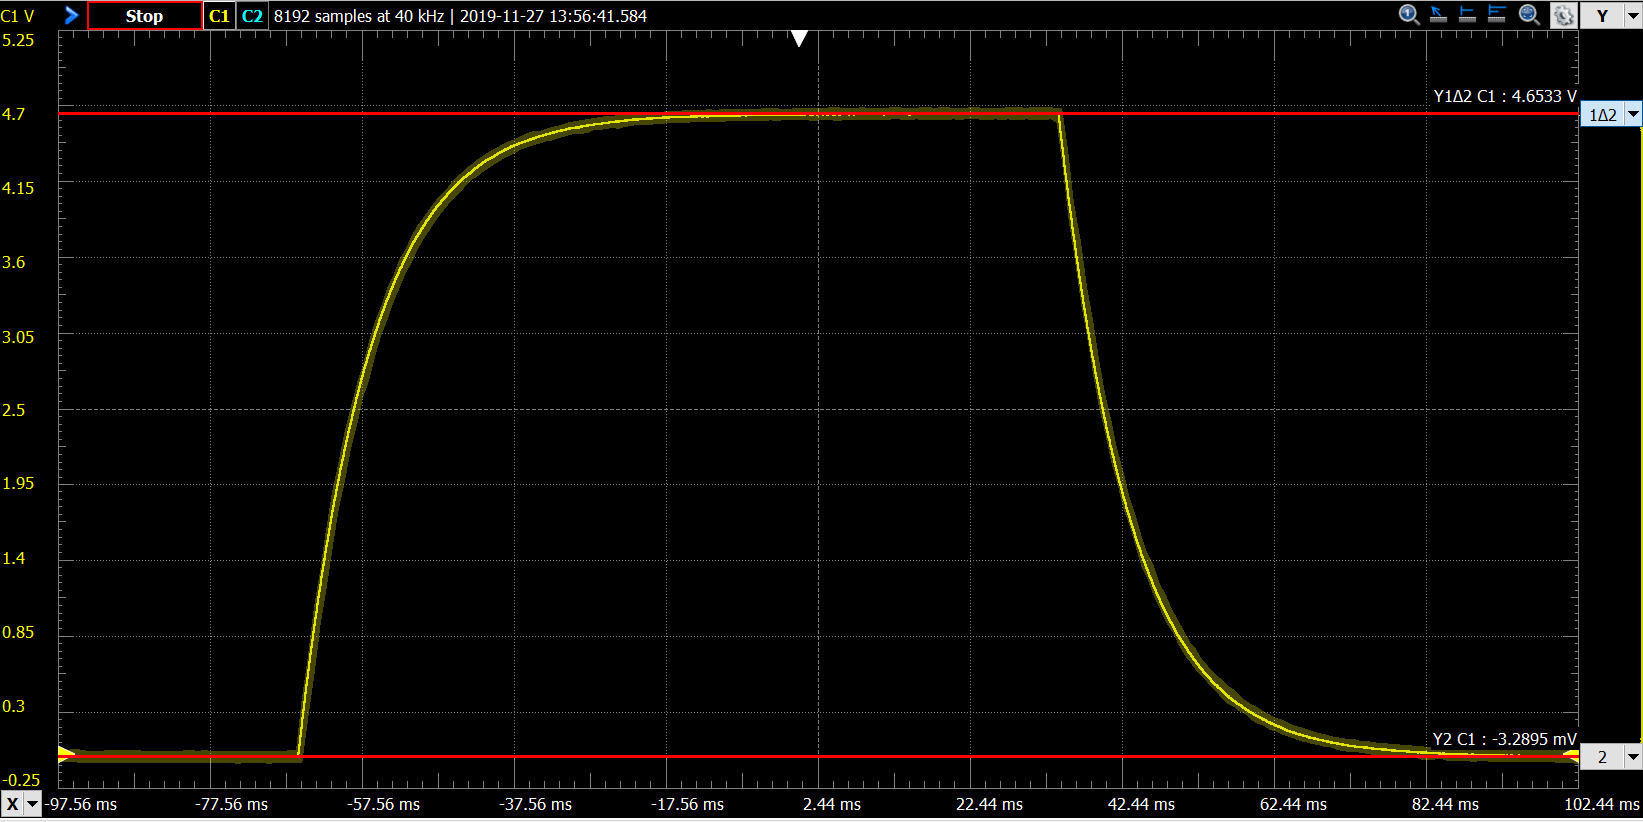
\includegraphics[height=5cm]{E_Tex/Rea_1_100_max}
\caption{Måling $V_{max}$ på 1. ordens lavpasfilter med 100k$Omega$}
\label{Rea_1_100_max}
\end{center}
\end{figure}
